%!TEX encoding=UTF-8 Unicode
\chapter{Memory Performance Analysis}

The results of our case study (\chap{perf}) showed that traditional performance analysis tools can help identify memory related performance issues.
Yet they are not able to tell precisely where, in terms of data structures, the issue occurs and thus it is still required to analyze the code manually.
As memory is often a performance bottleneck, several tools where developed to analyze performance in regards of the memory.

This chapter discuss memory analysis tools, first we present the specificities of recent memory subsystems and the usual mistakes that can generate performances drop in \sect{archi}.
Finally we present existing performance analysis tools related to memory in \sect{mem-tools} and describe how we could improve these tools in \sect{mem-cncl}.

\section{Architectural considerations}
\label{sec:archi}

Since a few decades, processor frequency increased significantly more than memory frequencies, resulting in a considerable gap between these two resources.
Indeed, retrieving one piece of data cost around $100$ \gls{CPU} cycles~\cite{Drepper07What}.
To mitigate this issue, the \glspl{CPU} embed a cache hierarchy that allow to keep highly used data closer to them reducing the access time to around $10$ cycles.
These caches comes with several mechanisms to optimize their usage, yet a code written without considering memory pattern can easily defeat all these optimizations resulting in considerable performance lost.

\begin{figure}[htb]
    \centering
    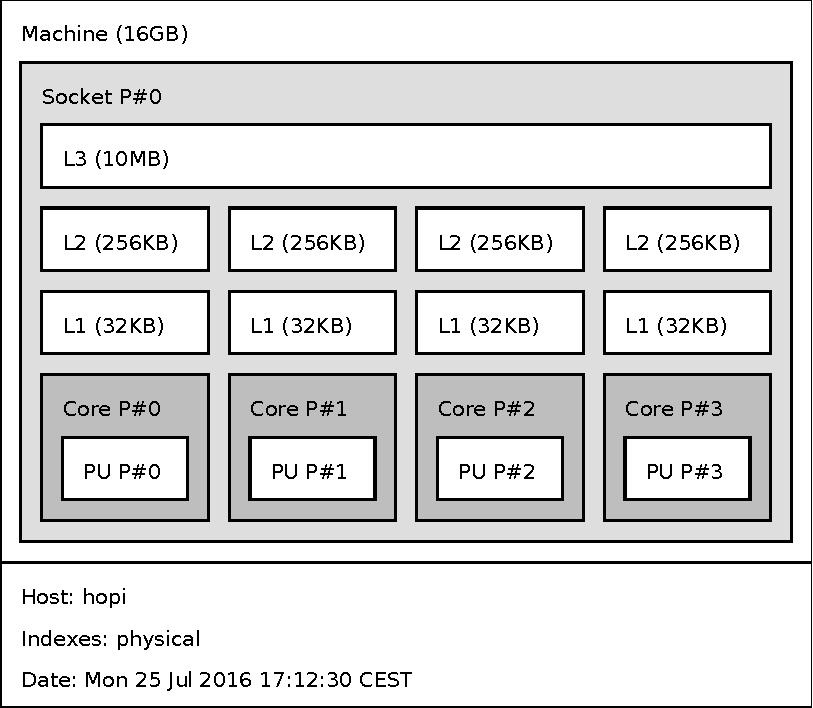
\includegraphics{hopi-topo}
    \caption[Simple cache hierarchy]{The Memory topology of a simple laptop computer.\\
        Figure generated by \emph{lstopo}}
    \label{fig:hopi-topo}
\end{figure}

\fig{osage-topo} presents the cache hierarchy of a laptop computer, it is composed of a \SI{8}{Gib} memory and one socket.
The \gls{CPU} is composed of two cores, four (hyper-)threads, and 3 level of caches.
The first level is private and split in two parts \texttt{L1d} for the data and \texttt{L1i} which store the instructions.
The second level only contains data and is still private, finally the third level is shared.

\begin{figure}[htb]
    \centering
    \missingfigure{Associative caches}
    \caption{Cache associativity}
    \label{fig:cache-assoc}
\end{figure}


\begin{figure}[htb]
    \centering
    \missingfigure{Illustration of naive mat mult, algo + memory pattern}
    \caption{Example of non linear memory accesses: the naïve matrix multiplication}
    \label{fig:mat-mult}
\end{figure}

\begin{figure}[htb]
    \centering
    \missingfigure{Illustration of two threads false sharing}
    \caption{Example of false sharing with two threads}
    \label{fig:false-sharing}
\end{figure}

\begin{figure}[htb]
    \centering
    \missingfigure{Bad alignment}
    \caption{Example of bad alignment resulting in prefetcher failure}
    \label{fig:bad-align}
\end{figure}

\begin{itemize}
    \item Memory Organisation
        \begin{itemize}
            \item Levels (hierarchy, example lstopo)
            \item Pages => Virtual memory, lazy load
            \item Cache lines for coherency
            \item Associativity
            \item Prefetcher
        \end{itemize}
    \item Usual issues
        \begin{itemize}
            \item False sharing
            \item Bad alignment / pattern change => prefetcher get lost
                \begin{itemize}
                    \item Garbage fetch (Remove useful stuff from cache
                    \item Several accesses for data that could be fetched at once
                \end{itemize}
            \item Linearity irregular acces (example fig: matmult)
            \item Cache garbage - piracy (Swann, related compass)
        \end{itemize}
    \item More parallelism => Several sockets => Contentions => \gls{NUMA}
        \begin{itemize}
            \item Remote accesses more costly
            \item Coherency highly costly as L3 not shared
            \item Need to split memory and bind thread / data
            \item Usual policy
                \begin{itemize}
                    \item First touch: beware of init
                    \item Interleave don't reduce the number of remote accesses, just balance them to reduce contention
                    \item Chunks by threads: Requires deep understanding of mem pattern + complex computations
                \end{itemize}
        \end{itemize}
    \item Importance of visualizing pattern
    \item Parenthesis: \gls{GPU} more complexe hierarchy, everything is mem oriented, code must be memory dependent, yet no tools to visualize mem pattern (yer)
\end{itemize}

\section{Existing Tools and Methodology}
\label{sec:mem-tools}

%% From Moca Paper, rewrite
Most performance analyses are based on hardware performance counters, which are CPU
register initially designed by CPU vendors to debug their prototypes. They contain
the count of specific events such as branch prediction misses or cache misses.
Theses counters are accessible directly  through the \texttt{Perf} driver
since Linux kernel $2.6.31$ but they are CPU and vendor dependent. Thus, higher
level libraries such as \emph{PAPI}~\cite{Weaver13PAPI} and
\emph{Likwid}~\cite{Treibig10LIKWID} were developed to ease their use.
In addition, these higher level libraries are able to derivate more abstract metrics. Several works propose to analyze memory 
by looking solely at the information collected through these
libraries~\cite{Majo13(Mis)understanding,
Jiang14Understanding,Bosch00Rivet,Weyers14Visualization,Tao01Visualizing,DeRose01Hardware}.
%
Several generic tools have been designed on top of hardware performance counters
to analyze and improve parallel applications performances, such as Intel's
VTune~\cite{Reinders05VTune}, Performance Counter
Monitor~(PCM)~\cite{Intel2012b}, the HPCToolkit~\cite{Adhianto10HPCTOOLKIT},
and AMD's CodeAnalyst~\cite{Drongowski2008}.
%
Although performance counters provide information about the memory use
(bandwith, volume of data transferred \ldots),  they consider the memory as
one huge entity and do not differentiate distinct addresses or at least
distinct pages. Thus, these methods are not able to locate issues in the memory.

Some tools see the memory as a set of pages, loosing information at a finer
granularity. This approximation enable to trace memory accesses at a reduced
cost. For instance, \gls{Tabarnac}~\cite{Beniamine15TABARNAC} uses a binary
instrumentation (based on Intel's Pin~\cite{Luk05Pin}) and traps each
memory access, but it only keeps one counter per page and per threads in order to
reduce its overhead. While this approach provides a deeper insight about the
memory use than hardware performance counters, it lacks temporal information.

Tracing all the memory accesses without information loss is nearly impossible as
almost each instruction can trigger a memory access in addition to its fetch. Nevertheless, several methods
can record a \emph{detailed} memory trace with a good \emph{precision}.
%
Budanur et al.~\cite{Budanur11Memory} use an instrumentation based tool to
collect all the memory accesses. They loose \emph{precision} by doing online compression and merging accesses
into a higher level model, but this is necessary to reduce both the trace size and its overhead.
Still, on a small matrix multiplication ($48*48$, 4 threads OpenMP) they already
slow the execution down by a factor of $50$.
% sampling:
Other methods, implemented by several
tools~\cite{Lachaize12MemProf,McCurdy10Memphis,Liu14Tool,Gimenez14Dissecting},
rely on hardware sampling such as AMD's Instruction Based Sampling
(IBS)~\cite{Drongowski07Instructionbased} or Intel Precise Event Based
Sampling (PEBS)~\cite{Levinthal2009}.  These methods provide \emph{incomplete}
sampling: some parts of the memory can be accessed without being noticed by
the tool if none of the associated instructions are part of the sampled
instructions.  Thus, it is possible that they ignore memory areas
less frequently accessed, but in which optimization could take place.
Applications sensitive to spurious performance
degradation, such as interactive applications, could be hindered by these
unnoticed accesses, despite their low frequency.
%
% Folding mechanisms: offtopic
%
% To make things practical, these sampling mechanisms monitor what they name an events set given by an instruction type along with some predicates.
% They can monitor several events sets at the same time but the number of monitored sets is limited by the hardware capabilities (number of available
% registers). Unfortunately, the number of existing events sets that relate to the memory hierarchy is large, because of its complexity.
% This makes difficult the task of tracing all the relevant memory accesses with just a single analysis.
% One way to lessen the impact of this limitation is to run several times the
% instrumentation and use advanced methods such as
% folding~\cite{Servat15Towards} to generate a more accurate summary trace.
% Nevertheless, this makes the instrumentation cost grow accordingly.
% Moreover, writing (and sometimes) using tools that relies on hardware mechanisms
% requires a deep knowledge of the processor. As processors evolve,
% such tools are hard to maintain and can quickly become outdated.
% We regard all these limitations as too constraining for a general purpose
% memory analysis tool.

Other studies rely on hardware modifications, either actual or
simulated~\cite{Bao08HMTT,Martonosi92MemSpy}.  Although they are eventually
able to collect more \emph{precise} traces efficiently, these techniques are limited
to hardware developers. Indeed, to use these hardware extensions one has
either to obtain (or build) a prototype or to use a suitable simulator. Such
configuration is not realistic for general purpose memory analysis.

Finally, page faults interception can provide useful online information about
memory usage. Such a mechanism has been used in several existing works : in
parallel garbage collectors~\cite{Boehm91Mostly}, in memory
checkpointing~\cite{Heo05Spaceefficient} or in the domain of virtualization to
provide the hypervisor with information about the memory usage of the guest
OS~\cite{Jones06Geiger}. However, page faults only occur when caused by
predetermined events in the system (copy-on-write, paging, ...). Thus, just intercepting existing page
faults only provide an approximate view of the memory use. To improve this method,
it is also possible to fake invalid
pages at regular intervals in order to generate false
page faults~\cite{Bae12Dynamic,Diener13CommunicationBased}.  These false page
faults are just triggered during regular memory accesses, that would not have
caused a page fault if the page were not faked as invalid. The advantage is
that they create additional events for the monitoring tool to collect, thus
more \emph{precision}, but the set of faked invalid pages has to be known and
maintained by the monitoring tool.

As a final note, tools close to our proposal do not use false page faults injection and only need to store the location of memory pages and the threads that access them.
As a consequence, they require a relatively small data structure in memory for their own usage.
In this study we present \gls{Moca}, a new \emph{complete} memory trace collection system, based on page
fault interception and false page faults injection, able to capture \emph{precisely} the temporal evolution of memory accesses performed by a multithreaded
application.
To reach a satisfying \emph{precision}, our tool has to maintain in memory both the trace data and
the set of faked invalid pages. Overall, storing and exploiting efficiently these data within the kernel space and outputting them in real time to the user space
is a challenge and is the main contribution of our work.

\section{Conclusions}
\label{sec:mem-cncl}

Need global info / temporal evolution
% vim: et si sta lbr  sw=4 ts=4 spelllang=en_us
